\documentclass[aspectratio=169]{beamer}
\usetheme{Madrid}
\usecolortheme{default}

\usepackage{amsmath,amssymb}
\usepackage{bm}
\usepackage{booktabs}
\usepackage{tikz}
\usetikzlibrary{arrows.meta,positioning,calc,fit,shapes.geometric}

\title{Bayesian Inference}
\subtitle{A concise introduction for graduate students in quantitative fields}
\author{Generated self-contained Beamer presentation}
\date{\today}

\newcommand{\E}{\mathbb{E}}
\newcommand{\Var}{\mathrm{Var}}
\newcommand{\Prb}{\mathbb{P}}
\newcommand{\Normal}{\mathcal{N}}
\newcommand{\BetaD}{\mathrm{Beta}}
\newcommand{\Binom}{\mathrm{Binomial}}
\newcommand{\Bern}{\mathrm{Bernoulli}}
\newcommand{\iid}{\stackrel{\mathrm{iid}}{\sim}}

\begin{document}

\begin{frame}
  \titlepage
\end{frame}

\begin{frame}{Learning goals}
\begin{itemize}
  \item Interpret Bayesian inference as coherent updating of uncertainty.
  \item Distinguish the roles of the prior, likelihood, posterior, and predictive distribution.
  \item Work through two conjugate examples: Beta--Binomial and Normal--Normal.
  \item Understand how Bayesian intervals, prediction, computation, and model checking differ from frequentist analogs.
\end{itemize}
\vspace{0.5em}
\begin{block}{Core idea}
Unknown quantities are treated as random variables, and observed data update beliefs through Bayes' rule.
\end{block}
\end{frame}

\begin{frame}{Why Bayesian inference?}
\begin{columns}[T,onlytextwidth]
\column{0.57\textwidth}
\begin{itemize}
  \item Quantifies uncertainty directly about parameters of interest.
  \item Naturally combines prior knowledge with new evidence.
  \item Produces full distributions, not just point estimates.
  \item Handles prediction and sequential learning in a unified framework.
\end{itemize}

\column{0.4\textwidth}
\centering
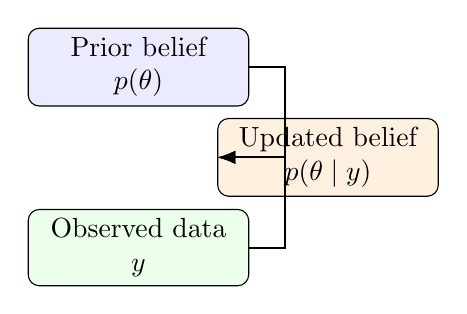
\begin{tikzpicture}[>=Latex, node distance=1.3cm]
  \tikzstyle{box}=[draw, rounded corners, align=center, minimum width=2.8cm, minimum height=0.9cm, fill=blue!8]
  \node[box] (prior) {Prior belief\\$p(\theta)$};
  \node[box, below=of prior, fill=green!8] (data) {Observed data\\$y$};
  \node[box, right=1.0cm of $(prior)!0.5!(data)$, fill=orange!12] (post) {Updated belief\\$p(\theta\mid y)$};
  \draw[->, thick] (prior.east) -- ++(0.45,0) |- (post.west);
  \draw[->, thick] (data.east) -- ++(0.45,0) |- (post.west);
\end{tikzpicture}
\end{columns}
\end{frame}

\begin{frame}{Bayes' theorem}
\begin{block}{Posterior distribution}
\[
  p(\theta\mid y)=\frac{p(y\mid\theta)\,p(\theta)}{p(y)},
  \qquad
  p(y)=\int p(y\mid\theta)p(\theta)\,d\theta.
\]
\end{block}

\begin{columns}[T,onlytextwidth]
\column{0.55\textwidth}
\begin{itemize}
  \item $p(\theta)$: \alert{prior} encodes beliefs before data.
  \item $p(y\mid\theta)$: \alert{likelihood} measures compatibility of $\theta$ with the data.
  \item $p(y)$: \alert{evidence} normalizes the posterior.
  \item $p(\theta\mid y)$: \alert{posterior} combines prior information and data.
\end{itemize}

\column{0.42\textwidth}
\begin{block}{Working proportionality}
In practice we often use
\[
  p(\theta\mid y)\propto p(y\mid\theta)p(\theta),
\]
and ignore $p(y)$ until normalization or sampling.
\end{block}
\end{columns}
\end{frame}

\begin{frame}{The Bayesian workflow}
\centering
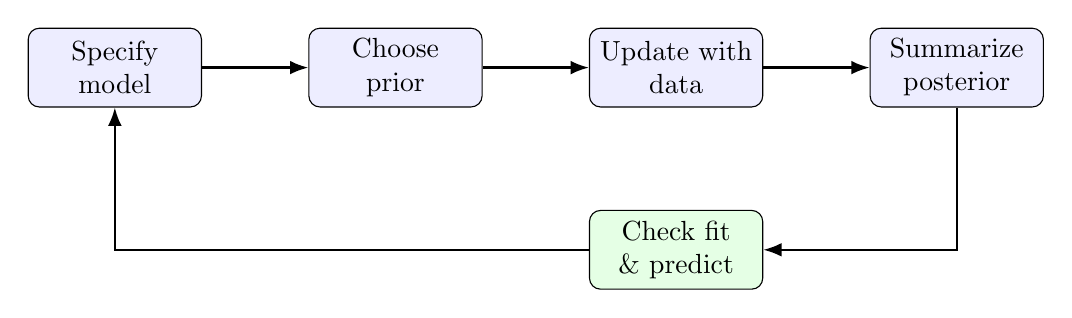
\begin{tikzpicture}[>=Latex, node distance=1.35cm]
  \tikzstyle{stage}=[draw, rounded corners, align=center, minimum width=2.2cm, minimum height=1.0cm, fill=blue!7]
  \node[stage] (model) {Specify\\model};
  \node[stage, right=of model] (prior) {Choose\\prior};
  \node[stage, right=of prior] (update) {Update with\\data};
  \node[stage, right=of update] (summ) {Summarize\\posterior};
  \node[stage, below=1.3cm of update, fill=green!10] (check) {Check fit \\\& predict};

  \draw[->, thick] (model) -- (prior);
  \draw[->, thick] (prior) -- (update);
  \draw[->, thick] (update) -- (summ);
  \draw[->, thick] (summ) |- (check);
  \draw[->, thick] (check.west) -| (model.south);
\end{tikzpicture}

\vspace{0.8em}
\begin{itemize}
  \item Bayesian analysis is iterative: model building and model checking form a loop.
  \item Posterior predictive checks often reveal misfit even when parameter estimates look reasonable.
\end{itemize}
\end{frame}

\begin{frame}{Example 1: Beta--Binomial model}
Suppose $y$ successes are observed in $n$ Bernoulli trials with success probability $\theta$.
\[
  y\mid\theta \sim \Binom(n,\theta),
  \qquad
  p(y\mid\theta)\propto \theta^y(1-\theta)^{n-y}.
\]
Choose a Beta prior:
\[
  \theta \sim \BetaD(\alpha,\beta),
  \qquad
  p(\theta)\propto \theta^{\alpha-1}(1-\theta)^{\beta-1}.
\]

\begin{block}{Conjugacy}
The posterior is in the same family as the prior, which makes updating algebraically simple.
\end{block}
\end{frame}

\begin{frame}{Closed-form update and interpretation}
Combining likelihood and prior gives
\[
  p(\theta\mid y)\propto \theta^{y+\alpha-1}(1-\theta)^{n-y+\beta-1},
\]
so that
\[
  \theta\mid y \sim \BetaD(\alpha+y,\beta+n-y).
\]

\begin{columns}[T,onlytextwidth]
\column{0.52\textwidth}
\begin{block}{Posterior mean}
\[
  \E[\theta\mid y]=\frac{\alpha+y}{\alpha+\beta+n}.
\]
It is a weighted average of the prior mean $\alpha/(\alpha+\beta)$ and the sample proportion $y/n$.
\end{block}

\column{0.44\textwidth}
\centering
\vspace{-0.9em}
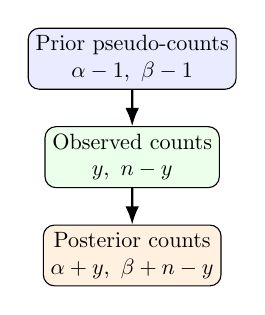
\begin{tikzpicture}[>=Latex, node distance=0.58cm, scale=0.8, transform shape]
  \tikzstyle{mini}=[draw, rounded corners, align=center, minimum width=2.45cm, minimum height=0.62cm]
  \node[mini, fill=blue!8] (prior) {Prior pseudo-counts\\$\alpha-1,\ \beta-1$};
  \node[mini, below=of prior, fill=green!8] (data) {Observed counts\\$y,\ n-y$};
  \node[mini, below=of data, fill=orange!12] (post) {Posterior counts\\$\alpha+y,\ \beta+n-y$};
  \draw[->, thick] (prior) -- (data);
  \draw[->, thick] (data) -- (post);
\end{tikzpicture}
\end{columns}
\end{frame}

\begin{frame}{Numerical update example}
Assume a prior centered at $0.50$ with moderate strength:
\[
  \theta \sim \BetaD(4,4).
\]
Observe $y=16$ successes in $n=20$ trials. Then
\[
  \theta\mid y \sim \BetaD(20,8).
\]

\begin{columns}[T,onlytextwidth]
\column{0.55\textwidth}
\begin{itemize}
  \item Prior mean: $4/(4+4)=0.50$.
  \item Sample proportion: $16/20=0.80$.
  \item Posterior mean: $20/28\approx 0.714$.
  \item The posterior shrinks the raw sample proportion toward the prior mean.
\end{itemize}

\column{0.4\textwidth}
\begin{block}{Interpretation}
The prior acts like extra observations, so Bayesian estimates often stabilize noisy small-sample problems.
\end{block}
\end{columns}
\end{frame}

\begin{frame}{Example 2: Normal mean with known variance}
Suppose
\[
  y_i \mid \theta \iid \Normal(\theta,\sigma^2),
  \qquad
  \theta \sim \Normal(\mu_0,\tau_0^2),
\]
with known sampling variance $\sigma^2$.

\begin{block}{Posterior distribution}
\[
  \theta\mid y \sim \Normal(\mu_n,\tau_n^2),
\]
where
\[
  \tau_n^2=\left(\frac{1}{\tau_0^2}+\frac{n}{\sigma^2}\right)^{-1},
  \qquad
  \mu_n=\tau_n^2\left(\frac{\mu_0}{\tau_0^2}+\frac{n\bar y}{\sigma^2}\right).
\]
\end{block}
The posterior mean is a precision-weighted average of the prior mean and sample mean.
\end{frame}

\begin{frame}{Posterior summaries and interval estimates}
Once we have $p(\theta\mid y)$, common summaries include:
\[
  \text{posterior mean }\E[\theta\mid y],
  \qquad
  \text{MAP }\arg\max_{\theta} p(\theta\mid y),
  \qquad
  \text{posterior variance }\Var(\theta\mid y).
\]

\begin{columns}[T,onlytextwidth]
\column{0.5\textwidth}
\begin{block}{Credible interval}
A $95\%$ credible interval $[a,b]$ satisfies
\[
  \Prb(\theta\in[a,b]\mid y)=0.95.
\]
This is a probability statement about the parameter given the observed data.
\end{block}

\column{0.47\textwidth}
\begin{block}{Frequentist confidence interval}
A $95\%$ confidence interval is a procedure whose long-run coverage is $95\%$ over repeated samples.
\end{block}
\end{columns}
\end{frame}

\begin{frame}{Posterior predictive distribution}
Prediction integrates over parameter uncertainty:
\[
  p(\tilde y\mid y)=\int p(\tilde y\mid\theta)p(\theta\mid y)\,d\theta.
\]

\begin{columns}[T,onlytextwidth]
\column{0.56\textwidth}
\begin{itemize}
  \item This is crucial: predictions should reflect uncertainty in both noise and parameters.
  \item In the Beta--Binomial model, the predictive probability of success on the next trial is
  \[
    \Prb(\tilde y=1\mid y)=\E[\theta\mid y]=\frac{\alpha+y}{\alpha+\beta+n}.
  \]
  \item Posterior predictive checks compare replicated data $\tilde y$ with observed data $y$.
\end{itemize}

\column{0.38\textwidth}
\centering
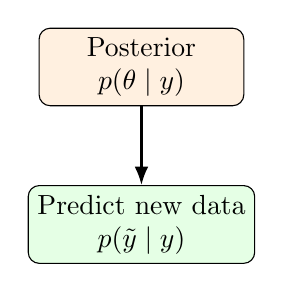
\begin{tikzpicture}[>=Latex, node distance=1.0cm]
  \tikzstyle{box}=[draw, rounded corners, align=center, minimum width=2.6cm, minimum height=0.85cm]
  \node[box, fill=orange!12] (post) {Posterior\\$p(\theta\mid y)$};
  \node[box, below=of post, fill=green!10] (pred) {Predict new data\\$p(\tilde y\mid y)$};
  \draw[->, thick] (post) -- (pred);
\end{tikzpicture}
\end{columns}
\end{frame}

\begin{frame}{Hierarchical models and partial pooling}
Bayesian models scale naturally to grouped data. For groups $j=1,\dots,J$:
\[
  y_{ij}\mid\theta_j \sim p(y_{ij}\mid\theta_j),
  \qquad
  \theta_j\mid\mu,\tau^2 \sim \Normal(\mu,\tau^2).
\]

\begin{columns}[T,onlytextwidth]
\column{0.52\textwidth}
\begin{itemize}
  \item Group-specific parameters borrow strength from one another.
  \item Small groups are shrunk more strongly toward the population mean.
  \item This often improves estimation and prediction relative to no pooling or complete pooling.
\end{itemize}

\column{0.42\textwidth}
\centering
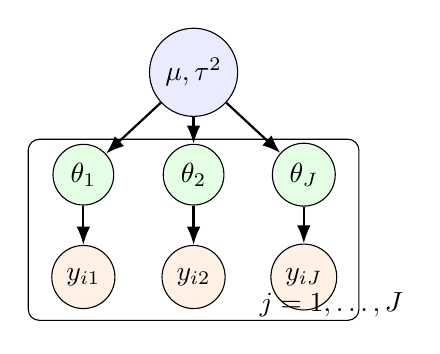
\begin{tikzpicture}[>=Latex]
  \node[draw, circle, fill=blue!8] (mu) at (0,1.8) {$\mu,\tau^2$};
  \node[draw, circle, fill=green!10] (t1) at (-1.4,0.5) {$\theta_1$};
  \node[draw, circle, fill=green!10] (t2) at (0,0.5) {$\theta_2$};
  \node[draw, circle, fill=green!10] (t3) at (1.4,0.5) {$\theta_J$};
  \node[draw, circle, fill=orange!10] (y1) at (-1.4,-0.8) {$y_{i1}$};
  \node[draw, circle, fill=orange!10] (y2) at (0,-0.8) {$y_{i2}$};
  \node[draw, circle, fill=orange!10] (y3) at (1.4,-0.8) {$y_{iJ}$};
  \draw[->, thick] (mu) -- (t1);
  \draw[->, thick] (mu) -- (t2);
  \draw[->, thick] (mu) -- (t3);
  \draw[->, thick] (t1) -- (y1);
  \draw[->, thick] (t2) -- (y2);
  \draw[->, thick] (t3) -- (y3);
  \draw[rounded corners] (-2.1,-1.35) rectangle (2.1,0.95);
  \node at (1.75,-1.15) {$j=1,\dots,J$};
\end{tikzpicture}
\end{columns}
\end{frame}

\begin{frame}{When closed forms fail: computation}
Many useful posteriors are not analytically tractable.

\begin{block}{Common computational strategies}
\begin{itemize}
  \item \textbf{MCMC}: constructs a Markov chain whose stationary distribution is the posterior.
  \item \textbf{Hamiltonian Monte Carlo}: efficient for high-dimensional continuous parameters.
  \item \textbf{Variational inference}: turns inference into optimization for faster approximations.
\end{itemize}
\end{block}

\begin{block}{Diagnostics matter}
Check convergence, effective sample size, Monte Carlo standard errors, and sensitivity to priors.
\end{block}
\end{frame}

\begin{frame}{Model checking and sensitivity analysis}
\begin{columns}[T,onlytextwidth]
\column{0.58\textwidth}
\begin{itemize}
  \item \textbf{Posterior predictive checks}: compare observed summaries $T(y)$ to replicated summaries $T(\tilde y)$.
  \item \textbf{Residual structure}: look for patterns left unexplained by the model.
  \item \textbf{Prior sensitivity}: ask whether substantive conclusions change under reasonable alternative priors.
  \item \textbf{Decision relevance}: assess whether posterior uncertainty is small enough for the scientific or policy question.
\end{itemize}

\column{0.37\textwidth}
\centering
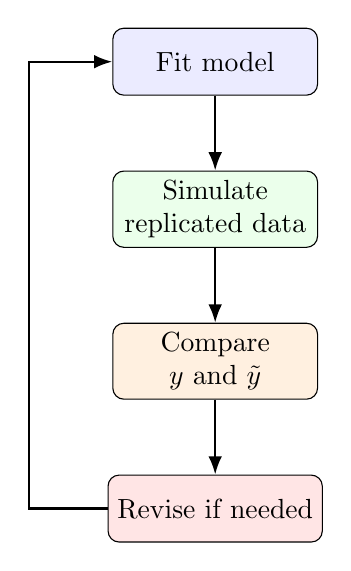
\begin{tikzpicture}[>=Latex, node distance=0.95cm]
  \tikzstyle{box}=[draw, rounded corners, align=center, minimum width=2.6cm, minimum height=0.85cm]
  \node[box, fill=blue!8] (fit) {Fit model};
  \node[box, below=of fit, fill=green!8] (rep) {Simulate\\replicated data};
  \node[box, below=of rep, fill=orange!12] (cmp) {Compare\\$y$ and $\tilde y$};
  \node[box, below=of cmp, fill=red!10] (rev) {Revise if needed};
  \draw[->, thick] (fit) -- (rep);
  \draw[->, thick] (rep) -- (cmp);
  \draw[->, thick] (cmp) -- (rev);
  \draw[->, thick] (rev.west) -| ++(-1.0,0) |- (fit.west);
\end{tikzpicture}
\end{columns}
\end{frame}

\begin{frame}{Bayesian linear regression in one line}
For the Gaussian linear model
\[
  \bm y\mid\bm\beta,\sigma^2 \sim \Normal(X\bm\beta,\sigma^2 I),
\]
with Gaussian prior $\bm\beta\sim\Normal(\bm\beta_0,V_0)$, the posterior is also Gaussian:
\[
  V_n=(V_0^{-1}+X^TX/\sigma^2)^{-1},
  \qquad
  \bm\beta_n=V_n\left(V_0^{-1}\bm\beta_0+X^T\bm y/\sigma^2\right).
\]

\begin{block}{Why this matters}
This reveals a general pattern: regularization methods such as ridge regression can often be interpreted as Bayesian estimation with specific priors.
\end{block}
\end{frame}

\begin{frame}{Takeaways}
\begin{enumerate}
  \item Bayesian inference updates uncertainty via
  \[
    \text{posterior} \propto \text{likelihood} \times \text{prior}.
  \]
  \item Conjugate models build intuition; modern computation handles richer models.
  \item Credible intervals and predictive distributions are direct, interpretable posterior summaries.
  \item Good Bayesian practice includes prior choice, computation, model checking, and sensitivity analysis.
\end{enumerate}

\vspace{0.5em}
\begin{block}{Final message}
Bayesian inference is not only a formula; it is a workflow for learning from data under uncertainty.
\end{block}
\end{frame}

\end{document}
